\chapter{State of the Art}
\label{chap:soa}

\section{The Artificial Intelligence Spectrum}
%%Referencias a los tipos de modelos y a los modelos hibridos que hay y a los estudios quasifilosoficos sobre por que unos pisan a otros, reemplazan a otros, mejoran a otros, etc.

\begin{figure*}
    \centering
    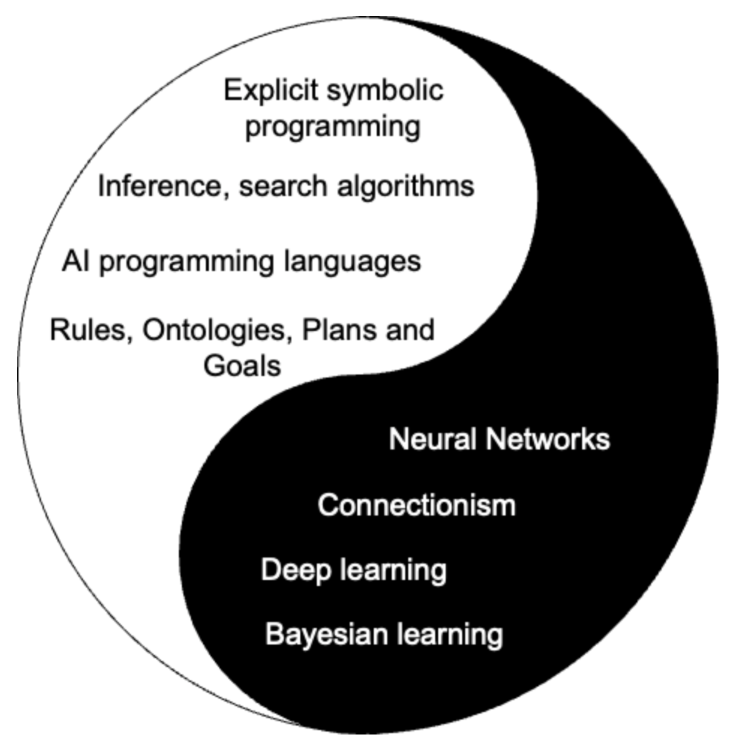
\includegraphics[width=.5\linewidth]{3_stateoftheart/figures/Lieberman_taxonomy.eps}
    \caption{AI Spectrum as depicted in \citep{lieberman_symbolic_nodate}}
    \label{fig:lieberman_tax}
\end{figure*}

Throughout the years, several categorizations have been proposed for the existing Artificial Intelligence (AI) models, each attending to a specific criteria. \citep{lieberman_symbolic_nodate} categorizes AI models considering their input in two categories: symbolic (also referred to as "classic AI") and subsymbolic. These two types are disjoint and complimentary to each other. \citep{lieberman_symbolic_nodate} depicts the AI spectrum as a \textit{yin-yang} (Figure \ref{fig:lieberman_tax}), where the flaws of one kind are compensated by the benefits of the other. While this categorization presents a simple and general overview on the existing AI models, it lacks a middle ground where hybrid approaches can be categorized. 

Opposite to this vision, where the focus is on the input, \citep{loyola-gonzalez_black-box_2019} envisions the AI spectrum from the perspective of the output. This taxonomy categorizes AI approaches as \textit{white-box} or \textit{black-box} considering whether the process that lead to a given output can be explained or not. The notation \textit{black-box} is used to describe those models whose inference process cannot be explain, which mainly applies to machine learning models.  \textit{Black-box} models can be subsequently grouped in: hyperplane-based (Support Vector Machines), neural networks (Convolutional Neural Networks, Graph Neural Networks), probability-based (Probabilistic Logic Networks) and instance-based (K-nearest neighbours). On the opposite side of this spectrum lie \textit{white-box} models, which relate to those approaches whose inference process can be understood and explain. Decision trees, rule-based systems or fuzzy logic are encompassed in this category.


\begin{figure}
    \centering
    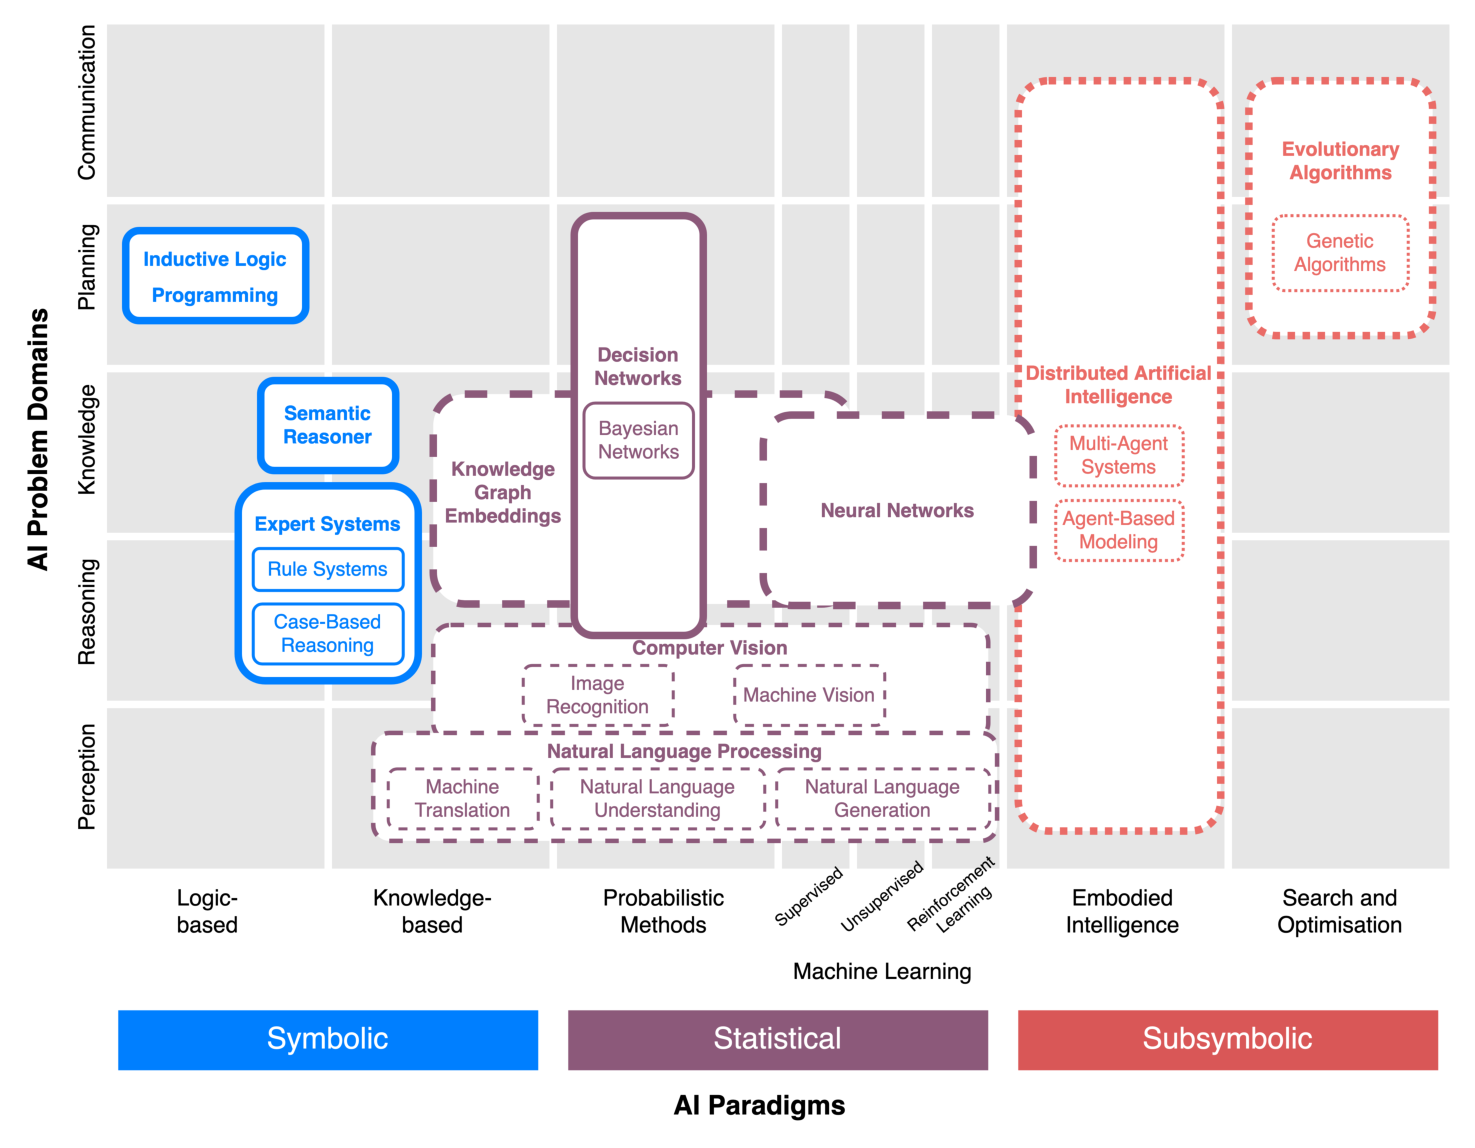
\includegraphics[width=\linewidth]{3_stateoftheart/figures/AI_Map.eps}
    \caption{Map of AI models combining the taxonomy of \citep{corea_ai_2019} with the taxonomy considered in this thesis. Symbolic, statistical and subsymbolic approaches are colour-coded in blue, purpe and red respectively. Knowledge-based and computational intelligent systems are coded in continuous and non-continuous lines, respectively. Dashed lines depict deep learning approaches, while dotted lines depict other computational intelligent approaches.}
    \label{fig:ai_map}
\end{figure}


More recently, \citep{corea_ai_2019} proposed a two dimensional categorization of AI technologies. Instead of considering the input or output of the model, this taxonomy focuses on the application domains of each paradigm and its reasoning paradigm. Figure \ref{fig:ai_map} portrays this categorization, where the Y-Axis comprises the existing problem domains, while the X-Axis encodes the three considered paradigms: symbolic, statistical and subsymbolic. While the taxonomy proposed by \citep{lieberman_symbolic_nodate} only considered the symbolic (blue) and subsymbolic (red) categories, \citep{corea_ai_2019} also considers the statistical (purple) models, as an in-between group between the two complimentary groups. Moreover, finer-grained subcategories can be distinguished inside each of the three main paradigms:
\begin{itemize}
    \item \textbf{Symbolic models:} As previously described, the term \textit{symbolic} describes AI paradigms that not only employ symbolic representations as input, but have an inference process that can be understood and explained by humans. Two finer grained types are identified inside this category: logic-based and knowledge-based.
    \item \textbf{Statistical models:} While the taxonomy proposed by \citep{lieberman_symbolic_nodate} only comprised symbolic and subsymbolic models, which are treated as analogous and complimentary kinds, this taxonomy distinguishes statistical models from purely subsymbolic models. These models employ mathematical tools for reasoning, and can be subsequently divided into probabilistic and machine lerning models.
    \item\textbf{Subsymbolic models:} According to this taxonomy, the term \textit{symbolic} refers to the absence of previous knowledge needed to function. Embodied intelligence models and search and optimisation models are grouped under this criterion.
\end{itemize}

The previous taxonomies provided categories that were fully disjoint and, therefore, each particular model needed to belong to exclusively one of the types. The taxonomy of \citep{corea_ai_2019} enables a higher degree of flexibility, as models can be applied under different problem domains as well as use different reasoning paradigms.
%%Taxonomias de la mas antigua a la mas moderna
\citep{hopgood_2009_knowledge-based} proposed a division of AI paradigms in two main categories: knowledge-based systems and computationally intelligent systems. Knowledge-based systems require explicit representations of knowledge in a symbolic form, while computationally intelligent systems use nature-inspired paradigms where no background knowledge is required to reason. This taxonomy can be merged with the taxonomy of \citep{corea_ai_2019}, providing a three-dimensional taxonomy as depicted in Figure \ref{fig:ai_map}. A third dimension depicting whether the paradigm can be classified as knowledge-based (continuous line) or computationally intelligent (discontinuous line). 

Deep Learning was introduced after \citep{hopgood_2009_knowledge-based} taxonomy was defined and, therefore, it did not cover these models. Therefore, a slight update on this base taxonomy is proposed to include deep learning models. Figure \ref{fig:ai_map} makes a distinction inside the computationally intelligent models, denoting in a dashed instead of a dotted line those paradigms that can be considered as deep learning. 

After combining the taxonomies presented in \citep{hopgood_2009_knowledge-based} and \citep{corea_ai_2019}, the final categorization of models is as follows:
\begin{itemize}
    \item \textbf{Knowledge-Based Systems:} These system fit almost perfectly the definition previously provided for the symbolic paradigms. Therefore, this category groups all the models that require from background expert knowledge to reason:
    \begin{itemize}
        \item \textit{Inductive Logic Programming (ILP):} This term was first introduced by \citep{Muggleton1991}, describing this field as "\textit{the area of AI which deals with the induction of hypothesised predicate definitions from examples and background knowledge}". ILP is one of the prime examples of symbolic learning, using fully expressive representations to encode logical clauses and knowledge, making the input, the output and the induction process fully explainable.
        \item \textit{Semantic Reasoners:} Instead of expressing background knowledge by means of logical clauses or predicates as in ILP, semantic reasoners use ontologies to encode background knowledge. Ontologies \citep{noy2001ontology} provide explicit specifications of conceptualizations which are shared and understood between humans and machines. Moreover, ontologies present a formal definition of classes (or types) and the properties and relations between those classes and their instances in a given domain. From the information encoded in an ontology, a semantic reasoner (also refered to as reasoning engine) can infer new axioms from the existing axioms.
        \item \textit{Expert Systems:} Formally, an expert system can be described as an AI system capable of emulating the decision-making process of a human expert of a given domain. These systems are composed by two differentiated parts: an inference engine and a knowledge base. The knowledge base encodes the facts, rules and background information needed. The inference engine applies the rules existing in the knowledge base to the known facts to infer new facts. \textit{Rule Systems} are the cornerstone of expert systems, using if-then clauses to infer new information from the already existing knowledge. As both facts and rules are encoded in a declarative way, the inference process can be fully understood and explained by humans. \elvitodo{A lo mejor esto hay que aumentarlo un poco}
        
        \textit{Case-Based Reasoning} (CBR) \citep{overview_cbr} is another example of expert system. In this case, the knowledge base is replaced by a case base, where a set of problem-solution tuples (or cases) are stored. CBR implements a continuous cycle, where the model improves overtime by including the knowledge acquired from the resolution of new problems, whose solutions are then stored in the case base. Therefore, the performance of the model improves overtime. A CBR model is composed by four distinct phases: retrieve, reuse, revise and retain. When a new problem enters the system, the retrieve phase is triggered, returning the most similar existing cases to the introduced one. From the most similar cases, a tailored solution for the input problem is devised on the reuse stage using the already-known solutions of the most similar cases. The proposed solution is then revised, determining whether it is suitable for the problem or not. If the solution satisfies the input problem, the newly-generated case is stored in the case base, and will serve for the resolution of subsequent problems.   
        
        \item \textit{Decision Networks,} also referred to as influence diagrams \citep{poole_2017_ai_foundations} are graphical representations of a finite and sequential decision problem. A decision network is generally composed by three types of nodes: chance, decision and utility nodes, which are assorted as a directed cyclic graph. \textit{Bayesian Networks} \citep{friedman_1997_bayesian} are the most common paradigm amongst decision networks. Based on the Bayes theorem, these decision networks model the conditional dependencies between variables, modelling the probability of each variable. Therefore, Bayesian networks can be used both to infer an outcome given the input variables as well as to determine the most feasible combination of variables that led to a giving output. As variables are explicitly declared and their probabilities are known, the inference process of Bayesian networks can be also fully understood by humans.
    \end{itemize}
    \item \textbf{Computational Intelligence:} Following the taxonomy from \citep{corea_ai_2019}, computational intelligence models cover both statistical and subsymbolic paradigms. As deep learning models are generally based on statistics, the remaining of the computational intelligence spectrum according to the proposed categorization comprises the following models:
    \begin{itemize}
        \item \textit{Multi-Agent Systems} (MAS) \citep{Ferber:1999:MSI:520715} are one of the most extended paradigms for the simulation of scenarios involving complex entities. These models comprise a set of self-organized intelligent agents which cooperate and interact to perform a given task. As it involves several independent components, there models are capable of solving complex tasks that can not be solved by single-task systems. Agents of a MAS are autonomous, act locally and are independent of each other. 
        \item \textit{Evolutionary Algorithms} \cite{GALVAN2003573} are heuristic-based systems inspired by natural evolution mechanisms. They are mostly applied to combinatorial problems, as they can greatly reduce the time required to go through the search space while still reaching a optimal solution. Typically, an evolutionary algorithm comprises four steps: initialization, selection, operation and termination. These stages are closely related to those happening in natural selection. Therefore, those candidate solutions that better fit the problem will replicate and proliferate, while those inadequate will be slowly discarded throughout the evolution process. 
    \end{itemize}
    \item \textbf{Deep Learning Approaches:}
    \begin{itemize}
        \item \textit{Neural Networks:}
        \item \textit{Knowledge Graph Embeddings:}
        \item \textit{Computer Vision Approaches:}
        \item \textit{Natural Language Processing:}
    \end{itemize}

\end{itemize}

%%Nuestra taxonomia y cuales son cada uno 


\section{Design Methods for Hybrid Learning Systems}

%%Modelos hibridos, por que se reemplazan unos a otros, beneficios, aproximaciones, clasificaciones dentro de este marco. 

%%Patrones de diseño con boxologia

\section{Deep Learning Enhanced Knowledge-Based Systems}
%%Ejemplos de esto. Extraemos limitaciones y cositas y criterios.

\section{Background Knowledge Integration for Deep Learning Models}
%%Same

\section{Explainable Artificial Intelligence}
%%Same same

\section{Conclusions and Limitations of the State-of-the-Art}
%Tabla resumen con todas las limitaciones encontradas 